\begin{prob}
	در محیط
	\texttt{prob}
	می‌توان صورت مسئله یا پاسخ آن را نوشت.  در انتهای سؤال یک خط افقی رسم می‌شود و در ابتدای آن یک خط‌چین. به طور پیش‌فرض سؤال‌ها از سؤال ۱ شروع شده و یکی یکی اضافه می‌شوند.
	
\end{prob}
\begin{sol}
	محیط
	\texttt{sol},
	در انتهای آخرین خط متنی که درون آن قرار دارد یک 
	$ \blacksquare $
	قرار می‌دهد.\\	
	همچنین پس از اتمام متن، یک خط افقی رسم می‌کند. اگر قصد دارید از این قابلیت استفاده کنید، به یاد داشته باشید که 
	\lr{\texttt{\textbackslash{solutiontrue}}}
	را در ابتدای 
	\texttt{configs.tex}
	جای‌گذاری کنید.
\end{sol}
\begin{probnum}{10}
	می‌توان با استفاده از محیط
	\texttt{probnum}
	سؤال با شمارهٔ دل‌خواه نوشت و پس از آن با استفاده از محیط 
	\texttt{prob}
	شمارش سؤالات به طور معمول خواهد بود.
	
\end{probnum}
\begin{prob}
	شماره‌گذاری سؤال‌ها به صورت عادی ادامه پیدا می‌کند.
	
\end{prob}
\begin{sol}
	
	\begin{customEnv}{محیط دل‌خواه}
		می‌توان از محیط
		\texttt{customEnv}
		برای مواردی مثل «لم»، «ادعا» و... استفاده کرد. به صورت پیش‌فرض این محیط بدون شماره‌گذاری است.
	\end{customEnv}
	\begin{customEnv}[]{محیط عددی}
		با استفاده از
		\texttt{[]}
		برای محیط
		\texttt{customEnv},
		محیط تعریف‌شده شماره‌گذاری می‌شود.
	\end{customEnv}
	\begin{customEnv}[]{محیط عددی}
		با استفادهٔ مجدد از یک محیط شماره‌گذاری‌شده، شمارهٔ آن افزایش می‌یابد. ‌می‌توان تا ۴ محیط عددی با اسم‌های مختلف تعریف کرد.
	\end{customEnv}
	برای سادگی جهت شماره‌گذاری فارسی، به جای حالت پیش‌فرض
	\LaTeX
	(یعنی آ ب ج...) می‌توان از محیط
	\texttt{faEnum}
	استفاده کرد که الفبای درست فارسی یعنی الف، ب، پ، ت و... را نمایش می‌دهد.
	\begin{faEnum}
		\item اولین مورد
		\item دومین مورد
		\item سومین مورد
	\end{faEnum}
	به‌طور پیش‌فرض این محیط یی پرانتز پس از الفبا قرار می‌دهد. می‌توان با
	\texttt{faEnum[-]}
	محیط را طوری تغییر داد که به جای پرانتز از خط تیره استفاده کند.
	\begin{faEnum}[-]
		\item اولین مورد
		\item دومین مورد
	\end{faEnum}
\end{sol}

\begin{figure}
	\centering
	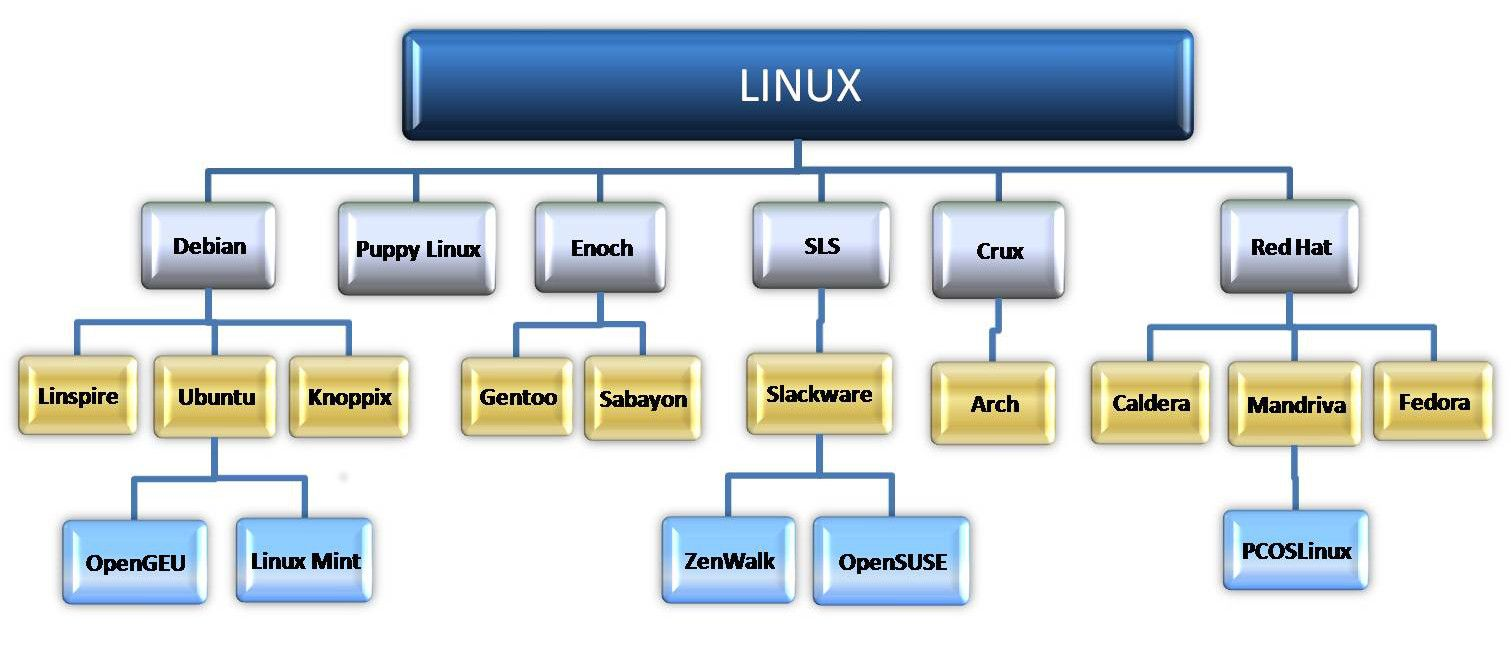
\includegraphics[width=1.0\linewidth]{image}
	\caption[عکس]{عکس}
	\label{fig:image}
\end{figure}
